% Options for packages loaded elsewhere
\PassOptionsToPackage{unicode}{hyperref}
\PassOptionsToPackage{hyphens}{url}
\PassOptionsToPackage{dvipsnames,svgnames,x11names}{xcolor}
%
\documentclass[
  letterpaper,
  DIV=11,
  numbers=noendperiod]{scrreprt}

\usepackage{amsmath,amssymb}
\usepackage{iftex}
\ifPDFTeX
  \usepackage[T1]{fontenc}
  \usepackage[utf8]{inputenc}
  \usepackage{textcomp} % provide euro and other symbols
\else % if luatex or xetex
  \usepackage{unicode-math}
  \defaultfontfeatures{Scale=MatchLowercase}
  \defaultfontfeatures[\rmfamily]{Ligatures=TeX,Scale=1}
\fi
\usepackage{lmodern}
\ifPDFTeX\else  
    % xetex/luatex font selection
\fi
% Use upquote if available, for straight quotes in verbatim environments
\IfFileExists{upquote.sty}{\usepackage{upquote}}{}
\IfFileExists{microtype.sty}{% use microtype if available
  \usepackage[]{microtype}
  \UseMicrotypeSet[protrusion]{basicmath} % disable protrusion for tt fonts
}{}
\makeatletter
\@ifundefined{KOMAClassName}{% if non-KOMA class
  \IfFileExists{parskip.sty}{%
    \usepackage{parskip}
  }{% else
    \setlength{\parindent}{0pt}
    \setlength{\parskip}{6pt plus 2pt minus 1pt}}
}{% if KOMA class
  \KOMAoptions{parskip=half}}
\makeatother
\usepackage{xcolor}
\setlength{\emergencystretch}{3em} % prevent overfull lines
\setcounter{secnumdepth}{5}
% Make \paragraph and \subparagraph free-standing
\makeatletter
\ifx\paragraph\undefined\else
  \let\oldparagraph\paragraph
  \renewcommand{\paragraph}{
    \@ifstar
      \xxxParagraphStar
      \xxxParagraphNoStar
  }
  \newcommand{\xxxParagraphStar}[1]{\oldparagraph*{#1}\mbox{}}
  \newcommand{\xxxParagraphNoStar}[1]{\oldparagraph{#1}\mbox{}}
\fi
\ifx\subparagraph\undefined\else
  \let\oldsubparagraph\subparagraph
  \renewcommand{\subparagraph}{
    \@ifstar
      \xxxSubParagraphStar
      \xxxSubParagraphNoStar
  }
  \newcommand{\xxxSubParagraphStar}[1]{\oldsubparagraph*{#1}\mbox{}}
  \newcommand{\xxxSubParagraphNoStar}[1]{\oldsubparagraph{#1}\mbox{}}
\fi
\makeatother

\usepackage{color}
\usepackage{fancyvrb}
\newcommand{\VerbBar}{|}
\newcommand{\VERB}{\Verb[commandchars=\\\{\}]}
\DefineVerbatimEnvironment{Highlighting}{Verbatim}{commandchars=\\\{\}}
% Add ',fontsize=\small' for more characters per line
\usepackage{framed}
\definecolor{shadecolor}{RGB}{241,243,245}
\newenvironment{Shaded}{\begin{snugshade}}{\end{snugshade}}
\newcommand{\AlertTok}[1]{\textcolor[rgb]{0.68,0.00,0.00}{#1}}
\newcommand{\AnnotationTok}[1]{\textcolor[rgb]{0.37,0.37,0.37}{#1}}
\newcommand{\AttributeTok}[1]{\textcolor[rgb]{0.40,0.45,0.13}{#1}}
\newcommand{\BaseNTok}[1]{\textcolor[rgb]{0.68,0.00,0.00}{#1}}
\newcommand{\BuiltInTok}[1]{\textcolor[rgb]{0.00,0.23,0.31}{#1}}
\newcommand{\CharTok}[1]{\textcolor[rgb]{0.13,0.47,0.30}{#1}}
\newcommand{\CommentTok}[1]{\textcolor[rgb]{0.37,0.37,0.37}{#1}}
\newcommand{\CommentVarTok}[1]{\textcolor[rgb]{0.37,0.37,0.37}{\textit{#1}}}
\newcommand{\ConstantTok}[1]{\textcolor[rgb]{0.56,0.35,0.01}{#1}}
\newcommand{\ControlFlowTok}[1]{\textcolor[rgb]{0.00,0.23,0.31}{\textbf{#1}}}
\newcommand{\DataTypeTok}[1]{\textcolor[rgb]{0.68,0.00,0.00}{#1}}
\newcommand{\DecValTok}[1]{\textcolor[rgb]{0.68,0.00,0.00}{#1}}
\newcommand{\DocumentationTok}[1]{\textcolor[rgb]{0.37,0.37,0.37}{\textit{#1}}}
\newcommand{\ErrorTok}[1]{\textcolor[rgb]{0.68,0.00,0.00}{#1}}
\newcommand{\ExtensionTok}[1]{\textcolor[rgb]{0.00,0.23,0.31}{#1}}
\newcommand{\FloatTok}[1]{\textcolor[rgb]{0.68,0.00,0.00}{#1}}
\newcommand{\FunctionTok}[1]{\textcolor[rgb]{0.28,0.35,0.67}{#1}}
\newcommand{\ImportTok}[1]{\textcolor[rgb]{0.00,0.46,0.62}{#1}}
\newcommand{\InformationTok}[1]{\textcolor[rgb]{0.37,0.37,0.37}{#1}}
\newcommand{\KeywordTok}[1]{\textcolor[rgb]{0.00,0.23,0.31}{\textbf{#1}}}
\newcommand{\NormalTok}[1]{\textcolor[rgb]{0.00,0.23,0.31}{#1}}
\newcommand{\OperatorTok}[1]{\textcolor[rgb]{0.37,0.37,0.37}{#1}}
\newcommand{\OtherTok}[1]{\textcolor[rgb]{0.00,0.23,0.31}{#1}}
\newcommand{\PreprocessorTok}[1]{\textcolor[rgb]{0.68,0.00,0.00}{#1}}
\newcommand{\RegionMarkerTok}[1]{\textcolor[rgb]{0.00,0.23,0.31}{#1}}
\newcommand{\SpecialCharTok}[1]{\textcolor[rgb]{0.37,0.37,0.37}{#1}}
\newcommand{\SpecialStringTok}[1]{\textcolor[rgb]{0.13,0.47,0.30}{#1}}
\newcommand{\StringTok}[1]{\textcolor[rgb]{0.13,0.47,0.30}{#1}}
\newcommand{\VariableTok}[1]{\textcolor[rgb]{0.07,0.07,0.07}{#1}}
\newcommand{\VerbatimStringTok}[1]{\textcolor[rgb]{0.13,0.47,0.30}{#1}}
\newcommand{\WarningTok}[1]{\textcolor[rgb]{0.37,0.37,0.37}{\textit{#1}}}

\providecommand{\tightlist}{%
  \setlength{\itemsep}{0pt}\setlength{\parskip}{0pt}}\usepackage{longtable,booktabs,array}
\usepackage{calc} % for calculating minipage widths
% Correct order of tables after \paragraph or \subparagraph
\usepackage{etoolbox}
\makeatletter
\patchcmd\longtable{\par}{\if@noskipsec\mbox{}\fi\par}{}{}
\makeatother
% Allow footnotes in longtable head/foot
\IfFileExists{footnotehyper.sty}{\usepackage{footnotehyper}}{\usepackage{footnote}}
\makesavenoteenv{longtable}
\usepackage{graphicx}
\makeatletter
\def\maxwidth{\ifdim\Gin@nat@width>\linewidth\linewidth\else\Gin@nat@width\fi}
\def\maxheight{\ifdim\Gin@nat@height>\textheight\textheight\else\Gin@nat@height\fi}
\makeatother
% Scale images if necessary, so that they will not overflow the page
% margins by default, and it is still possible to overwrite the defaults
% using explicit options in \includegraphics[width, height, ...]{}
\setkeys{Gin}{width=\maxwidth,height=\maxheight,keepaspectratio}
% Set default figure placement to htbp
\makeatletter
\def\fps@figure{htbp}
\makeatother
% definitions for citeproc citations
\NewDocumentCommand\citeproctext{}{}
\NewDocumentCommand\citeproc{mm}{%
  \begingroup\def\citeproctext{#2}\cite{#1}\endgroup}
\makeatletter
 % allow citations to break across lines
 \let\@cite@ofmt\@firstofone
 % avoid brackets around text for \cite:
 \def\@biblabel#1{}
 \def\@cite#1#2{{#1\if@tempswa , #2\fi}}
\makeatother
\newlength{\cslhangindent}
\setlength{\cslhangindent}{1.5em}
\newlength{\csllabelwidth}
\setlength{\csllabelwidth}{3em}
\newenvironment{CSLReferences}[2] % #1 hanging-indent, #2 entry-spacing
 {\begin{list}{}{%
  \setlength{\itemindent}{0pt}
  \setlength{\leftmargin}{0pt}
  \setlength{\parsep}{0pt}
  % turn on hanging indent if param 1 is 1
  \ifodd #1
   \setlength{\leftmargin}{\cslhangindent}
   \setlength{\itemindent}{-1\cslhangindent}
  \fi
  % set entry spacing
  \setlength{\itemsep}{#2\baselineskip}}}
 {\end{list}}
\usepackage{calc}
\newcommand{\CSLBlock}[1]{\hfill\break\parbox[t]{\linewidth}{\strut\ignorespaces#1\strut}}
\newcommand{\CSLLeftMargin}[1]{\parbox[t]{\csllabelwidth}{\strut#1\strut}}
\newcommand{\CSLRightInline}[1]{\parbox[t]{\linewidth - \csllabelwidth}{\strut#1\strut}}
\newcommand{\CSLIndent}[1]{\hspace{\cslhangindent}#1}

\KOMAoption{captions}{tableheading}
\makeatletter
\@ifpackageloaded{bookmark}{}{\usepackage{bookmark}}
\makeatother
\makeatletter
\@ifpackageloaded{caption}{}{\usepackage{caption}}
\AtBeginDocument{%
\ifdefined\contentsname
  \renewcommand*\contentsname{Table des matières}
\else
  \newcommand\contentsname{Table des matières}
\fi
\ifdefined\listfigurename
  \renewcommand*\listfigurename{Liste des Figures}
\else
  \newcommand\listfigurename{Liste des Figures}
\fi
\ifdefined\listtablename
  \renewcommand*\listtablename{Liste des Tables}
\else
  \newcommand\listtablename{Liste des Tables}
\fi
\ifdefined\figurename
  \renewcommand*\figurename{Figure}
\else
  \newcommand\figurename{Figure}
\fi
\ifdefined\tablename
  \renewcommand*\tablename{Tableau}
\else
  \newcommand\tablename{Tableau}
\fi
}
\@ifpackageloaded{float}{}{\usepackage{float}}
\floatstyle{ruled}
\@ifundefined{c@chapter}{\newfloat{codelisting}{h}{lop}}{\newfloat{codelisting}{h}{lop}[chapter]}
\floatname{codelisting}{Listing}
\newcommand*\listoflistings{\listof{codelisting}{Liste des Listings}}
\makeatother
\makeatletter
\makeatother
\makeatletter
\@ifpackageloaded{caption}{}{\usepackage{caption}}
\@ifpackageloaded{subcaption}{}{\usepackage{subcaption}}
\makeatother

\ifLuaTeX
\usepackage[bidi=basic]{babel}
\else
\usepackage[bidi=default]{babel}
\fi
\babelprovide[main,import]{french}
% get rid of language-specific shorthands (see #6817):
\let\LanguageShortHands\languageshorthands
\def\languageshorthands#1{}
\ifLuaTeX
  \usepackage{selnolig}  % disable illegal ligatures
\fi
\usepackage{bookmark}

\IfFileExists{xurl.sty}{\usepackage{xurl}}{} % add URL line breaks if available
\urlstyle{same} % disable monospaced font for URLs
\hypersetup{
  pdftitle={Traitement d'images satellites avec Python},
  pdfauthor={Philippe Apparicio; Yacine Bouroubi; Samuel Foucher; Mickaël Germain},
  pdflang={fr},
  colorlinks=true,
  linkcolor={blue},
  filecolor={Maroon},
  citecolor={Blue},
  urlcolor={Blue},
  pdfcreator={LaTeX via pandoc}}


\title{Traitement d'images satellites avec Python}
\usepackage{etoolbox}
\makeatletter
\providecommand{\subtitle}[1]{% add subtitle to \maketitle
  \apptocmd{\@title}{\par {\large #1 \par}}{}{}
}
\makeatother
\subtitle{Première édition}
\author{Philippe Apparicio \and Yacine Bouroubi \and Samuel
Foucher \and Mickaël Germain}
\date{2024-09-27}

\begin{document}
\maketitle

\renewcommand*\contentsname{Table des matières}
{
\hypersetup{linkcolor=}
\setcounter{tocdepth}{2}
\tableofcontents
}

\bookmarksetup{startatroot}

\chapter*{Préface}\label{pruxe9face}
\addcontentsline{toc}{chapter}{Préface}

\markboth{Préface}{Préface}

\renewcommand{\partname}{} % Réinitialiser partie

\textbf{Résumé~:} Ce livre vise à décrire une panoplie de méthodes de
traitement d'images satellites avec le langage Python. Celles et ceux
souhaitant migrer progressivement d'un autre logiciel d'imagerie et de
télédétection vers Python trouveront dans cet ouvrage les éléments pour
une transition en douceur. La philosophie de ce livre est de donner
toutes les clefs de compréhension et de mise en œuvre des méthodes
abordées dans Python. La présentation des méthodes est basée sur une
approche compréhensive et intuitive plutôt que mathématique, sans pour
autant négliger la rigueur mathématique ou statistique.

\textbf{Remerciements~:} Ce manuel a été réalisé avec le soutien de la
fabriqueREL. Fondée en 2019, la fabriqueREL est portée par divers
établissements d'enseignement supérieur du Québec et agit en
collaboration avec les services de soutien pédagogique et les
bibliothèques. Son but est de faire des ressources éducatives libres
(REL) le matériel privilégié en enseignement supérieur au Québec.

\textbf{Maquette de la page couverture et identité graphique du livre~:}
Andrés Henao Florez.

\textbf{Mise en page~:} Philippe Apparicio et Marie-Hélène Gadbois Del
Carpio.

\textbf{Révision linguistique~:} Denise Latreille.

© Philippe Apparicio, Yacine Bouroubi, Samuel Foucher et Mickël Foucher.

\textbf{Pour citer cet ouvrage~:} Apparicio P., Bouroubi, Y., Foucher,
S. et M. Germain (2024). \emph{Traitement d'images satellites avec
Python}. Université de Sherbrooke, Département de géomatique appliquée.
fabriqueREL. Licence CC~BY-SA.


\includegraphics[width=0.8\textwidth,height=\textheight]{images/introduction/CouvertureP2.png}\hfill

\section*{Un manuel sous la forme d'une ressource éducative
libre}\label{sect001}
\addcontentsline{toc}{section}{Un manuel sous la forme d'une ressource
éducative libre}

\markright{Un manuel sous la forme d'une ressource éducative libre}

\textbf{Pourquoi un manuel sous licence libre?}

Les logiciels libres sont aujourd'hui très répandus. Comparativement aux
logiciels propriétaires, l'accès au code source permet à quiconque de
l'utiliser, de le modifier, de le dupliquer et de le partager. Le
logiciel Python, dans lequel sont mises en œuvre les méthodes de
traitement d'images satellites décrites dans ce livre, est d'ailleurs à
la fois un langage de programmation et un logiciel libre (sous la
licence publique générale
\href{https://fr.wikipedia.org/wiki/Licence_publique_g\%C3\%A9n\%C3\%A9rale_GNU}{GNU
GPL2}). Par analogie aux logiciels libres, il existe aussi des
\textbf{ressources éducatives libres (REL)} «~dont la licence accorde
les permissions désignées par les 5R (\textbf{Retenir --- Réutiliser ---
Réviser --- Remixer --- Redistribuer}) et donc permet nécessairement la
modification~»
(\href{https://fabriquerel.org/rel/}{\textbf{\emph{fabriqueREL}}}). La
licence de ce livre, CC BY-SA (figure~\ref{fig-Licence}), permet donc
de~:

\begin{itemize}
\item
  \textbf{Retenir}, c'est-à-dire télécharger et imprimer gratuitement le
  livre. Notez qu'il aurait été plutôt surprenant d'écrire un livre
  payant sur un logiciel libre et donc gratuit. Aussi, nous aurions été
  très embarrassés que des personnes étudiantes avec des ressources
  financières limitées doivent payer pour avoir accès au livre, sans
  pour autant savoir préalablement si le contenu est réellement adapté à
  leurs besoins.
\item
  \textbf{Réutiliser}, c'est-à-dire utiliser la totalité ou une section
  du livre sans limitation et sans compensation financière. Cela permet
  ainsi à d'autres personnes enseignantes de l'utiliser dans le cadre
  d'activités pédagogiques.
\item
  \textbf{Réviser}, c'est-à-dire modifier, adapter et traduire le
  contenu en fonction d'un besoin pédagogique précis puisqu'aucun manuel
  n'est parfait, tant s'en faut! Le livre a d'ailleurs été écrit
  intégralement dans R avec \href{https://quarto.org/}{Quatro}.
  Quiconque peut ainsi télécharger gratuitement le code source du livre
  sur
  \href{https://github.com/SerieBoldR/MethodesAnalyseSpatiale}{github}
  et le modifier à sa guise (voir l'encadré intitulé \emph{Suggestions
  d'adaptation du manuel}).
\item
  \textbf{Remixer}, c'est-à-dire «~combiner la ressource avec d'autres
  ressources dont la licence le permet aussi pour créer une nouvelle
  ressource intégrée~»
  (\href{https://fabriquerel.org/rel/}{\textbf{\emph{fabriqueREL}}}).
\item
  \textbf{Redistribuer}, c'est-à-dire distribuer, en totalité ou en
  partie le manuel ou une version révisée sur d'autres canaux que le
  site Web du livre (par exemple, sur le site Moodle de votre université
  ou en faire une version imprimée).
\end{itemize}

La licence de ce livre, CC BY-SA (figure~\ref{fig-Licence}), oblige donc
à~:

\begin{itemize}
\tightlist
\item
  Attribuer la paternité de l'auteur dans vos versions dérivées, ainsi
  qu'une mention concernant les grandes modifications apportées, en
  utilisant la formulation suivante~:
\end{itemize}

Apparicio Philippe, Yacine Bouroubi, Samuel Foucher et Mickaël Foucher
(2024). \emph{Traitement d'images satellites : }. Université de
Sherbrooke, Département de géomatique appliquée. fabriqueREL. Licence
CC~BY-SA.

\begin{itemize}
\tightlist
\item
  Utiliser la même licence ou une licence similaire à toutes versions
  dérivées.
\end{itemize}

\begin{figure}

\centering{

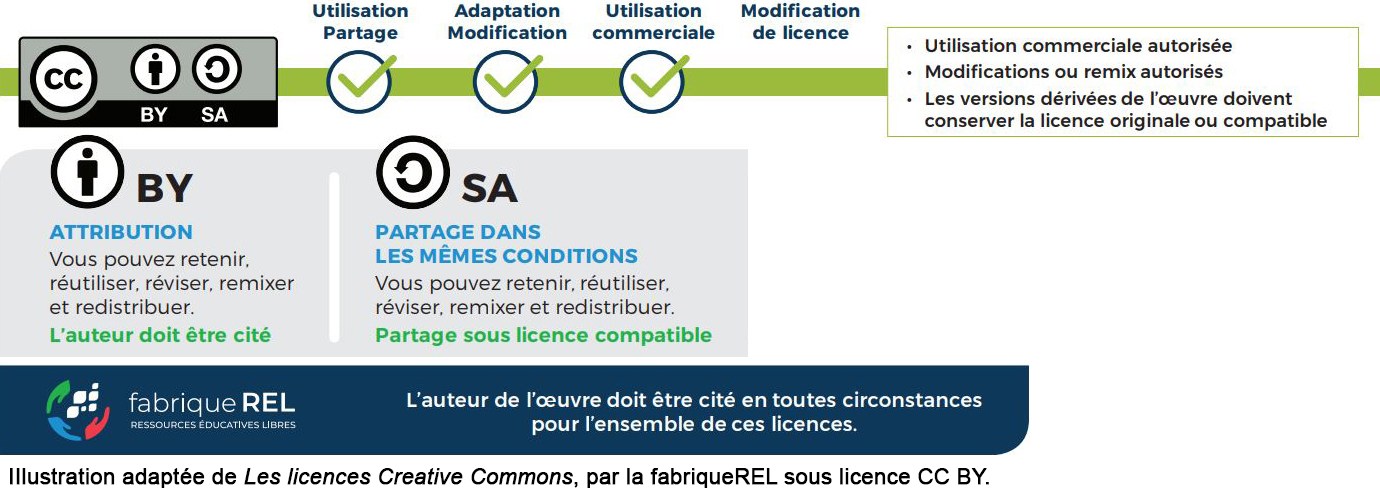
\includegraphics[width=0.8\textwidth,height=\textheight]{images/introduction/Licence.JPG}

}

\caption{\label{fig-Licence}Licence Creative Commons du livre}

\end{figure}%

\textbf{Suggestions d'adaptation du manuel}

Pour chaque méthode d'analyse spatiale abordée dans le livre, une
description détaillée et une mise en œuvre dans Python sont disponibles.
Par conséquent, plusieurs adaptations du manuel sont possibles~:

\begin{itemize}
\item
  Conserver uniquement les chapitres sur les méthodes ciblées dans votre
  cours.
\item
  En faire une version imprimée et la distribuer aux personnes
  étudiantes.
\item
  Modifier la description d'une ou de plusieurs méthodes en effectuant
  les mises à jour directement dans les chapitres.
\item
  Insérer ses propres jeux de données dans les sections intitulées
  \emph{Mise en œuvre dans Python}.
\item
  Modifier les tableaux et figures.
\item
  Ajouter une série d'exercices.
\item
  Modifier les quiz de révision.
\item
  Rédiger un nouveau chapitre.
\item
  Modifier des syntaxes en Python. Plusieurs \emph{librairies} Python
  peuvent être utilisées pour mettre en œuvre telle ou telle méthode.
  Ces derniers évoluent aussi très vite et de nouvelles
  \emph{librairies} sont proposées fréquemment! Par conséquent, il peut
  être judicieux de modifier une syntaxe Python du livre en fonction de
  ses habitudes de programmation en Python (utilisation d'autres
  \emph{librairies} que ceux utilisés dans le manuel par exemple) ou de
  bien mettre à jour une syntaxe à la suite de la parution d'une
  nouvelle \emph{librairie} plus performante ou intéressante.
\item
  Toute autre adaptation qui permet de répondre au mieux à un besoin
  pédagogique.
\end{itemize}

\section*{Comment lire ce manuel?}\label{sect002}
\addcontentsline{toc}{section}{Comment lire ce manuel?}

\markright{Comment lire ce manuel?}

Le livre comprend plusieurs types de blocs de texte qui en facilitent la
lecture.

\textbf{Bloc \emph{packages}}

Habituellement localisé au début d'un chapitre, il comprend la liste des
\emph{packages} Python utilisés pour un chapitre.

\textbf{Bloc objectif}

Il comprend une description des objectifs d'un chapitre ou d'une
section.

\textbf{Bloc notes}

Il comprend une information secondaire sur une notion, une idée abordée
dans une section.

\textbf{Bloc pour aller plus loin}

Il comprend des références ou des extensions d'une méthode abordée dans
une section.

\textbf{Bloc astuce}

Il décrit un élément qui vous facilitera la vie~: une propriété
statistique, un \emph{package}, une fonction, une syntaxe Python.

\textbf{Bloc attention}

Il comprend une notion ou un élément important à bien maîtriser.

\textbf{Bloc exercice}

Il comprend un court exercice de révision à la fin de chaque chapitre.

\section*{Comment utiliser les données du livre pour reproduire les
exemples?}\label{sect003}
\addcontentsline{toc}{section}{Comment utiliser les données du livre
pour reproduire les exemples?}

\markright{Comment utiliser les données du livre pour reproduire les
exemples?}

Ce livre comprend des exemples détaillés et appliqués dans R pour
chacune des méthodes abordées. Ces exemples se basent sur des jeux de
données structurés et mis à disposition avec le livre. Ils sont
disponibles sur le \emph{repo github} dans le sous-dossier
\texttt{data}, à l'adresse
\url{https://github.com/SerieBoldR/TraitementImagesVol1/tree/main/data}.

Une autre option est de télécharger le \emph{repo} complet du livre
directement sur \emph{github}
(\url{https://github.com/SerieBoldR/TraitementImagesVol1}) en cliquant
sur le bouton \texttt{Code}, puis le bouton \texttt{Download\ ZIP}
(figure~\ref{fig-downloaffromgit}). Les données se trouvent alors dans
le sous-dossier nommé \texttt{data}.

\begin{figure}

\centering{

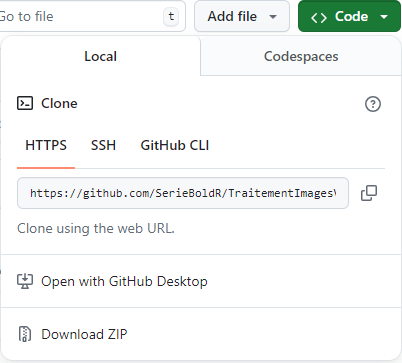
\includegraphics[width=0.4\textwidth,height=\textheight]{images/introduction/download_github.png}

}

\caption{\label{fig-downloaffromgit}Téléchargement de l'intégralité du
livre}

\end{figure}%

\section*{Structure du livre}\label{sect004}
\addcontentsline{toc}{section}{Structure du livre}

\markright{Structure du livre}

Le livre est organisé autour de quatre grandes parties.

\textbf{Partie 1. Importation et manipulation de données spatiales.}
Dans cette première partie, nous voyons comment importer, manipuler,
cartographier et exporter des données spatiales dans R, principalement
avec les \emph{packages} \texttt{sf} pour les données vectorielles,
\texttt{terra} pour les données matricielles (images) et \texttt{tmap}
pour la cartographie (chapitre~\ref{sec-chap01}). Maîtriser les notions
abordées dans ce chapitre constitue une étape préalable et indispensable
à tout projet d'analyse spatiale. D'une part, avant d'analyser des
données spatiales, il convient de les structurer (importation et
manipulation) et de les explorer (cartographie). D'autre part, une fois
la ou les méthodes d'analyse spatiale mises en œuvre, il convient de
cartographier les résultats finaux et de les exporter au besoin dans un
format de données géographiques (shapefile (\texttt{shp}), GeoPackage
(\texttt{GPKG}), GeoJSON (\texttt{geojson}), sqlite (\texttt{sqlite}),
GeoTiff, etc.).

\textbf{Partie 2. Transformations des données spatiales}. Cette
troisième partie comprend deux chapitres~: les transformations
spectrales (chapitre~\ref{sec-chap03}) et les transformations spatiales
(chapitre~\ref{sec-chap04}).

\textbf{Partie 3. Classifications d'images.} Cette troisième partie
comprend deux chapitres~: les classifications supervisées
(chapitre~\ref{sec-chap05}) et non supervisées
(chapitre~\ref{sec-chap06}).

\textbf{Partie 4. Données massives}. Cette quatrième et dernière partie
comprend un seul chapitre qui est dédié aux plateformes de mégadonnes
chapitre~\ref{sec-chap07}, notammment Google Earth Engine.

\section*{Remerciements}\label{sect005}
\addcontentsline{toc}{section}{Remerciements}

\markright{Remerciements}

De nombreuses personnes ont contribué à l'élaboration de ce manuel.

Ce projet a bénéficié du soutien pédagogique et financier de la
\href{https://fabriquerel.org/}{\textbf{\emph{fabriqueREL}}} (ressources
éducatives libres). Les différentes rencontres avec le comité de suivi
nous ont permis de comprendre l'univers des ressources éducatives libres
(REL) et notamment leurs \href{https://fabriquerel.org/rel/}{fameux 5R}
(Retenir --- Réutiliser --- Réviser --- Remixer --- Redistribuer), de
mieux définir le besoin pédagogique visé par ce manuel, d'identifier des
ressources pédagogiques et des outils pertinents pour son élaboration.
Ainsi, nous remercions chaleureusement les membres de la
\emph{fabriqueREL} pour leur soutien inconditionnel~:

\begin{itemize}
\item
  Myriam Beaudet, bibliothécaire à l'Université de Sherbrooke.
\item
  Marianne Dubé, coordonnatrice de la fabriqueREL, Université de
  Sherbrooke.
\item
  Serge Piché, conseiller pédagogique, Université de Sherbrooke.
\item
  Claude Potvin, conseiller en formation, Service de soutien à
  l'enseignement, Université Laval.
\end{itemize}

Nous remercions chaleureusement les personnes étudiantes des cours
\textbf{à modifier plus tard} du
\href{https://www.usherbrooke.ca/admission/programme/271/baccalaureat-en-geomatiqueappliquee-a-lenvironnement/}{Baccalauréat
en géomatique appliquée à l'environnement} et du
\href{https://www.usherbrooke.ca/admission/programme/429/microprogramme-de-1er-cycleen-geomatique-appliquee/}{Microprogramme
de 1er cycle en géomatique appliquée} du
\href{https://www.usherbrooke.ca/geomatique/}{Département de géomatique
appliquée} de l'\href{https://www.usherbrooke.ca/}{Université de
Sherbrooke} de la session d'été 2023~: à modifier plus tard.

Nous remercions aussi les membres du comité de révision pour leurs
commentaires et suggestions très constructifs. Ce comité est composé de
quatre personnes étudiantes du
\href{https://www.usherbrooke.ca/geomatique/}{Département de géomatique
appliquée} de l'\href{https://www.usherbrooke.ca/}{Université de
Sherbrooke}~:

\begin{itemize}
\item
  À compléter plus tard.
\item
  À compléter plus tard.
\end{itemize}

Finalement, nous remercions Denise Latreille, réviseure linguistique et
chargée de cours à l'Université Sherbrooke, pour la révision du manuel.

\section*{Introduction aux images de télédétection}\label{sect006}
\addcontentsline{toc}{section}{Introduction aux images de télédétection}

\markright{Introduction aux images de télédétection}

L'imagerie numérique a pris une place importante dans notre vie de tous
les jours depuis une quinzaine d'année. Ces images sont prises
généralement au niveau du sol (imagerie proximale) avec seulement trois
couleurs dans le domaine de la vision humaine (rouge, vert et bleu).
Dans la suite du manuel, on parlera d'images du domaine de la vision par
ordinateur ou images en vision pour faire plus court.

Les images de télédétection ont des particularités et des propriétés qui
les différencient des images de tous les jours. On peut souligner au
moins cinq caractéristiques principales: 1. Les images sont
géoréférencées : Cela veut dire que pour chaque pixel nous pouvons y
associer une position géographique ou cartographique. 2. Le point de vue
est très différent : Ces images sont prises avec une vue d'en haut
(Nadir) ou oblique avec une distance qui peut être très grande (On parle
d'images distales). 3. Elles possèdent plus que 3 bandes : Contrairement
aux images en vision, les images de télédétection possèdent bien souvent
plus que 3 bandes. Il n'est pas rare de trouver 4 bandes (Pléiade), 13
bandes (Sentinel-2, Landsat) et même 200 bandes pour des capteurs
hyperspectraux. 4. Elles peuvent être calibrées : Les valeurs numérique
de l'image peuvent être converties en quantités physiques (luminance,
réflectance, section efficiace, etc.) via une fonction de calibration.
5. Elles sont de grande taille : Il n'est pas rare de manipuler des
images qui font plusieurs dizaines de milliers de pixels en dimension.

\subsection*{Ressources en ligne}\label{ressources-en-ligne}
\addcontentsline{toc}{subsection}{Ressources en ligne}

\subsection*{\texorpdfstring{Listes des \emph{librairies}
utilisés}{Listes des librairies utilisés}}\label{sect0071}
\addcontentsline{toc}{subsection}{Listes des \emph{librairies} utilisés}

Dans ce livre, nous utilisons de nombreux \emph{packages} Python que
vous pouvez installer avec le code ci-dessous.

\begin{Shaded}
\begin{Highlighting}[]
\ImportTok{import}\NormalTok{ sys}
\ImportTok{import}\NormalTok{ subprocess}
\ImportTok{import}\NormalTok{ pkg\_resources}

\CommentTok{\# Liste des packages}
\NormalTok{list\_packages }\OperatorTok{=}\NormalTok{ [}\StringTok{"pandas"}\NormalTok{, }\StringTok{"scikit{-}image"}\NormalTok{, }\StringTok{"matplotlib"}\NormalTok{, }
                 \StringTok{"geopandas"}\NormalTok{, }\StringTok{"rasterio"}\NormalTok{, }\StringTok{"folium"}\NormalTok{]}

\CommentTok{\# Packages non installés dans la liste}
\NormalTok{installed\_packages }\OperatorTok{=}\NormalTok{ \{pkg.key }\ControlFlowTok{for}\NormalTok{ pkg }\KeywordTok{in}\NormalTok{ pkg\_resources.working\_set\}}
\NormalTok{packages\_not\_installed }\OperatorTok{=}\NormalTok{ [pkg }\ControlFlowTok{for}\NormalTok{ pkg }\KeywordTok{in}\NormalTok{ list\_packages }\ControlFlowTok{if}\NormalTok{ pkg.lower() }\KeywordTok{not} \KeywordTok{in}\NormalTok{ installed\_packages]}

\CommentTok{\# Installation des packages manquants}
\ControlFlowTok{if}\NormalTok{ packages\_not\_installed:}
    \BuiltInTok{print}\NormalTok{(}\StringTok{"Installing missing packages..."}\NormalTok{)}
    \ControlFlowTok{for}\NormalTok{ package }\KeywordTok{in}\NormalTok{ packages\_not\_installed:}
\NormalTok{        subprocess.check\_call([sys.executable, }\StringTok{"{-}m"}\NormalTok{, }\StringTok{"pip"}\NormalTok{, }\StringTok{"install"}\NormalTok{, package])}
    \BuiltInTok{print}\NormalTok{(}\StringTok{"All packages installed successfully."}\NormalTok{)}
\ControlFlowTok{else}\NormalTok{:}
    \BuiltInTok{print}\NormalTok{(}\StringTok{"All required packages are already installed."}\NormalTok{)}
\end{Highlighting}
\end{Shaded}

\subsection*{Python 101}\label{sect0073}
\addcontentsline{toc}{subsection}{Python 101}

\begin{figure}

\centering{

\begin{Shaded}
\begin{Highlighting}[]
\ImportTok{import}\NormalTok{ numpy }\ImportTok{as}\NormalTok{ np}
\ImportTok{import}\NormalTok{ matplotlib.pyplot }\ImportTok{as}\NormalTok{ plt}

\NormalTok{r }\OperatorTok{=}\NormalTok{ np.arange(}\DecValTok{0}\NormalTok{, }\DecValTok{2}\NormalTok{, }\FloatTok{0.01}\NormalTok{)}
\NormalTok{theta }\OperatorTok{=} \DecValTok{2} \OperatorTok{*}\NormalTok{ np.pi }\OperatorTok{*}\NormalTok{ r}
\NormalTok{fig, ax }\OperatorTok{=}\NormalTok{ plt.subplots(}
\NormalTok{  subplot\_kw }\OperatorTok{=}\NormalTok{ \{}\StringTok{\textquotesingle{}projection\textquotesingle{}}\NormalTok{: }\StringTok{\textquotesingle{}polar\textquotesingle{}}\NormalTok{\} }
\NormalTok{)}
\NormalTok{ax.plot(theta, r)}
\NormalTok{ax.set\_rticks([}\FloatTok{0.5}\NormalTok{, }\DecValTok{1}\NormalTok{, }\FloatTok{1.5}\NormalTok{, }\DecValTok{2}\NormalTok{])}
\NormalTok{ax.grid(}\VariableTok{True}\NormalTok{)}
\NormalTok{plt.show()}
\end{Highlighting}
\end{Shaded}

}

\caption{\label{fig-polar}}

\end{figure}%

\bookmarksetup{startatroot}

\chapter*{À propos des auteurs}\label{auteurs}
\addcontentsline{toc}{chapter}{À propos des auteurs}

\markboth{À propos des auteurs}{À propos des auteurs}

\href{https://www.usherbrooke.ca/recherche/fr/specialistes/details/philippe.apparicio}{\textbf{Philippe
Apparicio}} est professeur titulaire au
\href{https://www.usherbrooke.ca/geomatique/}{Département de géomatique
appliquée} de l'\href{https://www.usherbrooke.ca/}{Université de
Sherbrooke}. Il y enseigne aux
\href{https://www.usherbrooke.ca/geomatique/etudes/programmes}{programmes
de 1\textsuperscript{er} et 2\textsuperscript{e} cycles de géomatique}
les cours \emph{Transport et mobilité durable}, \emph{Modélisation et
analyse spatiale} et \emph{Géomatique appliquée à la gestion urbaine}.
Durant les dernières années, il a offert plusieurs formations aux Écoles
d'été du Centre interuniversitaire québécois de statistiques sociales
(\href{https://www.ciqss.org/}{CIQSS}). Géographe de formation, ses
intérêts de recherche incluent la justice et l'équité environnementale,
la mobilité durable, les pollutions atmosphérique et sonore, et le vélo
en ville. Il a publié une centaine d'articles scientifiques dans
différents domaines des études urbaines et de la géographie mobilisant
la géomatique et l'analyse spatiale.

\href{https://www.usherbrooke.ca/geomatique/departement/personnel/personnel-enseignant/yacine-bouroubi}{\textbf{Yacine
Bouroubi}} est professeur titulaire au
\href{https://www.usherbrooke.ca/geomatique/}{Département de géomatique
appliquée} de l'\href{https://www.usherbrooke.ca/}{Université de
Sherbrooke}. Il y enseigne aux
\href{https://www.usherbrooke.ca/geomatique/etudes/programmes}{programmes
de 1\textsuperscript{er} et 2\textsuperscript{e} cycles de géomatique}
les cours \emph{Transport et mobilité durable}, \emph{Modélisation et
analyse spatiale} et \emph{Géomatique appliquée à la gestion urbaine}.
Durant les dernières années, il a offert plusieurs formations aux Écoles
d'été du Centre interuniversitaire québécois de statistiques sociales
(\href{https://www.ciqss.org/}{CIQSS}). Géographe de formation, ses
intérêts de recherche incluent la justice et l'équité environnementale,
la mobilité durable, les pollutions atmosphérique et sonore, et le vélo
en ville. Il a publié une centaine d'articles scientifiques dans
différents domaines des études urbaines et de la géographie mobilisant
la géomatique et l'analyse spatiale.

\href{https://www.usherbrooke.ca/recherche/fr/specialistes/details/samuel.foucher}{\textbf{Samuel
Foucher}} est professeur titulaire au
\href{https://www.usherbrooke.ca/geomatique/}{Département de géomatique
appliquée} de l'\href{https://www.usherbrooke.ca/}{Université de
Sherbrooke}. Il y enseigne aux
\href{https://www.usherbrooke.ca/geomatique/etudes/programmes}{programmes
de 1\textsuperscript{er} et 2\textsuperscript{e} cycles de géomatique}
les cours \emph{Transport et mobilité durable}, \emph{Modélisation et
analyse spatiale} et \emph{Géomatique appliquée à la gestion urbaine}.
Durant les dernières années, il a offert plusieurs formations aux Écoles
d'été du Centre interuniversitaire québécois de statistiques sociales
(\href{https://www.ciqss.org/}{CIQSS}). Géographe de formation, ses
intérêts de recherche incluent la justice et l'équité environnementale,
la mobilité durable, les pollutions atmosphérique et sonore, et le vélo
en ville. Il a publié une centaine d'articles scientifiques dans
différents domaines des études urbaines et de la géographie mobilisant
la géomatique et l'analyse spatiale.

\href{https://www.usherbrooke.ca/geomatique/departement/personnel/personnel-enseignant/mickael-germain}{\textbf{Mickaël
Germain}} est professeur titulaire au
\href{https://www.usherbrooke.ca/geomatique/}{Département de géomatique
appliquée} de l'\href{https://www.usherbrooke.ca/}{Université de
Sherbrooke}. Il y enseigne aux
\href{https://www.usherbrooke.ca/geomatique/etudes/programmes}{programmes
de 1\textsuperscript{er} et 2\textsuperscript{e} cycles de géomatique}
les cours \emph{Transport et mobilité durable}, \emph{Modélisation et
analyse spatiale} et \emph{Géomatique appliquée à la gestion urbaine}.
Durant les dernières années, il a offert plusieurs formations aux Écoles
d'été du Centre interuniversitaire québécois de statistiques sociales
(\href{https://www.ciqss.org/}{CIQSS}). Géographe de formation, ses
intérêts de recherche incluent la justice et l'équité environnementale,
la mobilité durable, les pollutions atmosphérique et sonore, et le vélo
en ville. Il a publié une centaine d'articles scientifiques dans
différents domaines des études urbaines et de la géographie mobilisant
la géomatique et l'analyse spatiale.

\part{Partie 1. Importation, manipulation et visualisation de données
spatiales}

\bookmarksetup{startatroot}

\chapter{Introduction au langage Python}\label{sec-chap00}

Dans ce chapitre, nous allons présenter quelques éléments essentiels du
langage Python qui nous seront utiles dans ce manuel. Python est un
langage très riche et peut aboutir à des projets logiciels très
sophistiqués. Il est important de comprendre que la programmation Python
n'est pas une fin en soit ici. Python est pour nous principalement un
outil de `scriptage' et de manipulation de la donnée.

Python, créé par
\href{https://en.wikipedia.org/wiki/Guido_van_Rossum}{Guido van Rossum}
en 1991, est un langage de programmation polyvalent et facile à
apprendre, souvent comparé à un couteau suisse numérique pour sa
simplicité et sa polyvalence. Comme un outil multifonction, Python peut
être utilisé pour une variété de tâches, du développement web à
l'analyse de données, en passant par l'intelligence artificielle.

\section{Les distributions}\label{les-distributions}

Il existe plusieurs
\href{https://wiki.python.org/moin/PythonDistributions}{distributions}
du langage Python, ces distributions sont comme différentes saveurs de
votre glace préférée - chacune a ses propres caractéristiques uniques,
mais elles sont toutes fondamentalement Python. Voici un aperçu des
principales distributions :

\begin{itemize}
\item
  \href{https://www.python.org/downloads/}{CPython} : C'est la
  distribution ``vanille'' officielle, comme la recette originale de
  Python. C'est le choix idéal pour la compatibilité et la conformité
  aux standards.
\item
  \href{https://www.anaconda.com/download}{Anaconda} : Pensez-y comme à
  un sundae tout garni. Il vient avec de nombreuses bibliothèques
  scientifiques préinstallées, idéal pour l'analyse de données et le
  machine learning.
\item
  \href{https://docs.anaconda.com/miniconda/miniconda-install/}{Miniconda}
  : est une distribution légère de Python qui vous permet d'ajouter les
  librairies au besoin.
\item
  PyPy : C'est comme une version turbo de Python, optimisée pour la
  vitesse.
\end{itemize}

Jython et IronPython : Ces versions sont comme des traducteurs,
permettant à Python de ``parler'' Java (Jython) ou .NET (IronPython).
Chaque distribution a ses forces, que ce soit la simplicité, la vitesse
ou des fonctionnalités spécifiques. Le choix dépend de vos besoins,
comme choisir entre une glace simple ou un banana split élaboré.

\section{Les styles de programmation en
Python}\label{les-styles-de-programmation-en-python}

Il existe plusieurs approches pour programmer en Python. La plus directe
est en version interactive en tapant \texttt{python} et de rentrer des
commandes ligne par ligne.

\subsection{Les outils de
programmation}\label{les-outils-de-programmation}

Un code python prend la forme d'un simple fichier texte avec l'extension
\texttt{.py} et peut être modifié avec un simple éditeur de texte.
Cependnant, il n'y aura pas de rétroactions immédiates de l'interpréteur
Python ce qui rend la correction d'erreurs (débogage) beaucoup plus
laborieux.

Un IDE (\emph{Integrated Developement Environnement}) est comme une
boîte à outils complète pour les programmeurs, vous trouverez :

\begin{itemize}
\item
  Un éditeur de texte amélioré pour écrire votre code, avec des
  fonctionnalités comme la coloration syntaxique qui rend le code plus
  lisible.
\item
  Un compilateur qui transforme votre code en instructions que
  l'ordinateur peut comprendre.
\item
  Un débogueur pour trouver et corriger les erreurs, tel un détective
  numérique.
\item
  Des outils d'automatisation qui effectuent des tâches répétitives,
  comme un assistant virtuel pour le codage.
\item
  L'accès à la documentation des différentes librairies.
\end{itemize}

Ces outils intégrés permettent aux développeurs de travailler plus
efficacement, en passant moins de temps à jongler entre différentes
applications et plus de temps à produire du code.

Voici quelques options populaires :

\begin{itemize}
\item
  \href{https://www.jetbrains.com/pycharm/}{PyCharm} : C'est un des
  outils les plus utilisés dans l'industrie. Il offre une multitude de
  fonctionnalités comme l'autocomplétion intelligente et le débogage
  intégré, idéal pour les grands projets. Cepednant, cet outil peut être
  assez gourmand en mémoire et en CPU.
\item
  \href{https://code.visualstudio.com/}{Visual Studio Code} : Gratuit,
  léger mais puissant, il est personnalisable avec des extensions pour
  Python.
\item
  \href{https://www.spyder-ide.org/}{Spyder} : Logiciel libre et
  gratuit, orienté vers les applications scientifiques.
\item
  \href{https://jupyter.org/}{Jupyter Notebooks} : Imaginez un cahier
  interactif pour le code. Idéal pour l'analyse de données et
  l'apprentissage, il permet de mélanger code, texte et visualisations.
  Des services gratuits dans le \textbf{cloud} sont disponibles comme
  Google Colab et Kaggle. Ces environnements sont néanmoins moins
  appropriées pour des grands projets et le débogage.
\item
  Sublime Text : C'est comme un stylo élégant et rapide. Léger et
  rapide, il est apprécié pour sa simplicité et sa vitesse. Le choix
  dépend de vos besoins, que vous soyez débutant ou développeur
  chevronné. L'important est de trouver l'éditeur qui vous convient le
  mieux pour coder confortablemen
\end{itemize}

\section{Bonnes pratiques}\label{bonnes-pratiques}

Python est un langage très dynamique, qui évolue constamment. Il est
fortement conseillé d'utiliser des environnements virtuels pour gérer
vos différentes librairies. Voici quelques bonnes pratiques à suivre :

\begin{enumerate}
\def\labelenumi{\arabic{enumi}.}
\item
  \textbf{N'installez par la dernière version de Python} : installez
  toujours une version ou deux qui précède
  \href{https://www.python.org/downloads/}{la dernière version}. Les
  versions trop récentes peuvent être instables. La version de python
  désirée peut être spécifiée au moment de la création d'un
  environnement virtuel (voir plus bas).
\item
  \textbf{Utilisez des environnements virtuels} : Pensez-y comme à des
  compartiments séparées pour chaque projet. Cela évite les conflits
  entre les différentes versions de bibliothèques et garde votre système
  propre.
\item
  \textbf{Vérifiez l'installation} : Après l'installation, ouvrez un
  terminal et tapez \texttt{python\ -\/-version} pour vous assurer que
  tout fonctionne correctement.
\end{enumerate}

\subsection{Création d'un environnement
virtuel}\label{cruxe9ation-dun-environnement-virtuel}

Il y a deux façons d'installer environnement virtuel selon votre
distribution de Python:

\begin{enumerate}
\def\labelenumi{\arabic{enumi}.}
\tightlist
\item
  \textbf{Option 1} : vous utilisez
  \href{https://www.anaconda.com/download}{Anaconda} ou
  \href{https://docs.anaconda.com/miniconda/miniconda-install/}{Miniconda},
  dans ce cas la commande \texttt{conda} est utilisée pour créer un
  environnement test avec Python 3.10:
\end{enumerate}

\begin{Shaded}
\begin{Highlighting}[]
\ExtensionTok{conda}\NormalTok{ env }\AttributeTok{{-}n}\NormalTok{ test python=3.10}
\ExtensionTok{conda}\NormalTok{ activate test}
\end{Highlighting}
\end{Shaded}

\begin{enumerate}
\def\labelenumi{\arabic{enumi}.}
\setcounter{enumi}{1}
\tightlist
\item
  \textbf{Option 2} : vous utilisez
  \href{https://www.python.org/downloads/}{CPython}
\end{enumerate}

\begin{Shaded}
\begin{Highlighting}[]
\ExtensionTok{conda}\NormalTok{ env }\AttributeTok{{-}n}\NormalTok{ test python=3.10}
\ExtensionTok{conda}\NormalTok{ activate test}
\end{Highlighting}
\end{Shaded}

Note: si vous utiliser des notebook jupyter, vous avez déjà un
environnement virtuel qui contient le serveur jupyter.

\section{Les structures de base}\label{les-structures-de-base}

Il y a essentiellement deux structures de données que Python manipule :
les listes et les dictionnaires.

\section{Les listes}\label{les-listes}

Les listes sont comme des boites extensibles où vous pouvez ranger
différents types d'objets :

\begin{itemize}
\item
  Représentées par des crochets : \texttt{{[}1,\ 2,\ 3,\ "python"{]}}.
\item
  Ordonnées et modifiables (mutables), vous pouvez récupérer une valeur
  par sa position avec \texttt{{[}{]}}.
\item
  Permettent les doublons (deux fois la même valeur).
\item
  Idéales pour stocker des collections d'éléments que vous voulez
  modifier
\end{itemize}

\subsection{Les tuples}\label{les-tuples}

Les tuples sont similaires aux listes, mais les boîtes sont scellées :

\begin{itemize}
\item
  Représentés par des parenthèses : \texttt{(1,\ 2,\ 3,\ "python")}.
\item
  Ordonnés mais non modifiables (immutables).
\item
  Permettent les doublons.
\item
  Souvent utilisé pour stocker des données qui ne doivent pas changer
  (comme des paramètres).
\end{itemize}

\subsection{Les ensembles (Sets)}\label{les-ensembles-sets}

Les ensembles sont comme des boites magiques qui ne gardent qu'un
exemplaire de chaque objet :

\begin{itemize}
\item
  Représentés par des accolades : \texttt{\{1,\ 2,\ 3\}}.
\item
  Non ordonnés et modifiables.
\item
  N'autorisent pas les doublons.
\item
  Utiles pour éliminer les doublons et effectuer des opérations
  mathématiques sur des ensembles.
\end{itemize}

\section{Dictionnaires}\label{dictionnaires}

Les dictionnaires sont comme des boites avec des étiquettes sur chcune
d'elle :

\begin{itemize}
\item
  Représentés par des accolades avec des paires clé-valeur :
  \texttt{\{"nom":\ "Python",\ "année":\ 1991\}}.
\item
  Non ordonnés et modifiables.
\item
  Les clés doivent être uniques, mais les valeurs peuvent être
  dupliquées
\item
  Utiles pour stocker des données associatives ou pour créer des tables
  de recherche rapide
\end{itemize}

\section{Progrmmation objet}\label{progrmmation-objet}

La programmation orientée objet (POO) en Python est comme construire
avec des blocs LEGO. Chaque objet est un bloc LEGO avec ses propres
caractéristiques (attributs) et capacités (méthodes). Les classes sont
les plans pour créer ces blocs. Par exemple, une classe ``Voiture''
pourrait avoir des attributs comme ``couleur'' et ``vitesse'', et des
méthodes comme ``démarrer'' et ``accélérer''.

Python rend la POO accessible avec des fonctionnalités conviviales :

\begin{enumerate}
\def\labelenumi{\arabic{enumi}.}
\item
  \textbf{Encapsulation} : Comme emballer un cadeau, elle cache les
  détails internes d'un objet.
\item
  \textbf{Héritage} : Permet de créer de nouvelles classes basées sur
  des classes existantes, comme un enfant héritant des traits de ses
  parents.
\item
  \textbf{Polymorphisme} : Permet à différents objets de répondre au
  même message de manière unique, comme si différents animaux
  répondaient différemment à ``fais du bruit''.
\end{enumerate}

Ces caractéristiques font de Python un excellent choix pour apprendre et
appliquer les concepts de la POO, rendant le code plus organisé et
réutilisable

\textbf{Liste des \emph{packages} utilisés dans ce chapitre}

\begin{itemize}
\tightlist
\item
  Pour importer et manipuler des fichiers géographiques~:

  \begin{itemize}
  \tightlist
  \item
    \texttt{sf} pour importer et manipuler des données vectorielles.
  \item
    \texttt{terra} pour importer et manipuler des données matricielles.
  \end{itemize}
\item
  Pour construire des cartes et des graphiques~:

  \begin{itemize}
  \tightlist
  \item
    \texttt{tmap} est certainement le meilleur \emph{package} pour la
    cartographie.
  \item
    \texttt{ggplot2} pour construire des graphiques.
  \end{itemize}
\end{itemize}

\section{Quiz de révision du
chapitre}\label{quiz-de-ruxe9vision-du-chapitre}

\section{Cahier de révision (notebook)}\label{sec-016}

\textbf{Notebook 1.} À compléter

\begin{Shaded}
\begin{Highlighting}[]
\CommentTok{\# ...}
\CommentTok{\# à compléter}
\end{Highlighting}
\end{Shaded}

\bookmarksetup{startatroot}

\chapter{Importation et manipulation de données
spatiales}\label{sec-chap01}

Dans le chapitre, nous abordons quelques formats d'images ainsi que leur
lecture.

\textbf{Liste des \emph{librairies} utilisées dans ce chapitre}

\begin{itemize}
\tightlist
\item
  Pour importer et manipuler des fichiers géographiques~:

  \begin{itemize}
  \tightlist
  \item
    \texttt{sf} pour importer et manipuler des données vectorielles.
  \item
    \texttt{Rasterio} pour importer et manipuler des données
    matricielles.
  \end{itemize}
\item
  Pour construire des cartes et des graphiques~:

  \begin{itemize}
  \tightlist
  \item
    \texttt{tmap} est certainement le meilleur \emph{package} pour la
    cartographie.
  \item
    \texttt{Matplotlib} pour construire des graphiques.
  \end{itemize}
\end{itemize}

\section{Bases de Quarto\ldots{}}\label{sec-010}

Voici comment faire une liste~:

\begin{itemize}
\tightlist
\item
  \textbf{texte en gras}
\item
  \emph{texte en italique}

  \begin{itemize}
  \tightlist
  \item
    \textbf{\emph{Gras et italique}}
  \end{itemize}
\item
  R\textsuperscript{2} et NO\textsubscript{2}
\item
  \textsc{Petites majuscules}
\item
  Pour un lien Web,
  \href{https://www.usherbrooke.ca/geomatique/}{Département de
  géomatique appliquée}.
\end{itemize}

Voici comment intégrer des équations LaTeX. La formule de la distance
euclidienne (équation~\ref{eq-DistEuc}). Pour écrire directement une
équation dans le texte, il suffit de \(E = mc^2\).

\begin{equation}\phantomsection\label{eq-DistLongLat}{
 d_{ij} = 2R \cdot \text{ arcsin} \left( \sqrt{\text{sin}^2 \left( \frac{\delta _i - \delta _j}{2} \right) + \text{cos }\delta _i \cdot \text{cos }\delta _j \cdot \text{sin}^2 \left( \frac{\phi _i - \phi _j}{2} \right)} \right)
}\end{equation}

\begin{equation}\phantomsection\label{eq-DistEuc}{
 d_{ij} = \sqrt{(x_i-x_j)^2+(y_i-y_j)^2}
}\end{equation}

\begin{itemize}
\tightlist
\item
  Intégrer une figure (image) et l'appeler dans le texte
  (figure~\ref{fig-downloaffromgit}). À la
  figure~\ref{fig-downloaffromgit}, \ldots{} Notez que la numérotation
  des figures, des tableaux, des équations est automatique.
\end{itemize}

\begin{figure}

\centering{

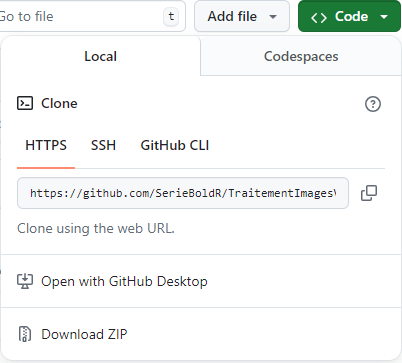
\includegraphics[width=0.4\textwidth,height=\textheight]{images/introduction/download_github.png}

}

\caption{\label{fig-downloaffromgit}Téléchargement de l'intégralité du
livre}

\end{figure}%

\begin{itemize}
\tightlist
\item
  Les références sont au format BibTeX. Par exemple, vous pouvez les
  télécharger de Google Scholar et les intégrer à la fin du fichier
  references.bib. Voici comment intégrer des références (Mather et Koch
  2022; Richards, Richards et al. 2022). Selon Ferdinand Boon et Guy
  Rochon (1992).
\end{itemize}

Le code R ci-dessous permet de faire un tableau dans un chunk! Pour
appeler le tableau (\textbf{?@tbl-TabMatricesSpatiales}).

\section{Importation d'images}\label{sec-011}

\subsection{Formats de données}\label{sec-0112}

\begin{itemize}
\tightlist
\item
  Format de type vision par ordinateur (RGB):

  \begin{itemize}
  \tightlist
  \item
    jpeg, png
  \end{itemize}
\item
  Format avec compression ou sans compression
\end{itemize}

Voici comment faire une liste

\begin{itemize}
\tightlist
\item
  Format RVB

  \begin{itemize}
  \tightlist
  \item
    jpeg
  \item
    png
  \end{itemize}
\item
  GeoTiff
\item
  COG
\item
  NetCDF
\item
  HDF5
\end{itemize}

\subsubsection{Formats de type RVB}\label{sec-01121}

Les premiers formats pour de l'imagerie à une bande (monochrome) et à
trois bandes (image couleur rouge-vert-bleu) sont issus du domaine des
sciences de l'ordinateur. On trouvera, entre autres, les formats pbm,
png et jpeg. Ces formats supportent peu de métadonnées dans un entête
(header) très limités. Ces formats restent très populaires dans le
domaine de la vision par ordinateur.

\subsubsection{Le format GeoTiff}\label{sec-01122}

Le format GeoTIFF est une extension du format TIFF (Tagged Image File
Format) qui permet d'incorporer des métadonnées géospatiales directement
dans un fichier image. Développé initialement par Dr.~Niles Ritter au
Jet Propulsion Laboratory de la
\href{https://www.earthdata.nasa.gov/esdis/esco/standards-and-practices/geotiff}{NASA}
dans les années 1990, GeoTIFF est devenu un standard de facto pour le
stockage et l'échange d'images géoréférencées dans les domaines de la
télédétection et des systèmes d'information géographique (SIG). Ce
format supporte plus que trois bandes aussi longtemps que ces bandes
sont de même dimension.

Le format GeoTIFF est très utilisé et est largement supporté par les
bibliothèques et logiciels géospatiaux, notamment GDAL (Geospatial Data
Abstraction Library), qui offre des capacités de lecture et d'écriture
pour ce format. Cette compatibilité étendue a contribué à son adoption
généralisée dans la communauté géospatiale.

\paragraph{Standardisation par l'OGC}\label{sec-011221}

Le standard GeoTIFF proposé par l'Open Geospatial Consortium (OGC) en
2019 formalise et étend les spécifications originales du format GeoTIFF,
offrant une norme robuste pour l'échange d'images géoréférencées. Cette
standardisation, connue sous le nom d'OGC GeoTIFF 1.1 (2019), apporte
plusieurs améliorations et clarifications importantes.

\subsubsection{Le format COG}\label{le-format-cog}

Une innovation récente dans l'écosystème GeoTIFF est le format ``Cloud
Optimized GeoTIFF'' (COG), conçu pour faciliter l'utilisation de
fichiers GeoTIFF hébergés sur des serveurs web HTTP. Le COG permet aux
utilisateurs et aux logiciels d'accéder à des parties spécifiques du
fichier sans avoir à le télécharger entièrement, ce qui est
particulièrement utile pour les applications basées sur le cloud.

\subsection{Métadonnées des images}\label{sec-0113}

\subsection{Données en géoscience}\label{sec-0114}

Calibration, unités, données manquantes, données éparses.

netcdf, xarray, GRIB.

Données météos, exemple avec SWOT.

\section{Importation de données vectorielles}\label{sec-012}

\subsection{\texorpdfstring{Importation d'un fichier
\emph{shapefile}}{Importation d'un fichier shapefile}}\label{sec-0121}

\subsection{\texorpdfstring{Importation d'une couche dans un
\emph{GeoPackage}}{Importation d'une couche dans un GeoPackage}}\label{sec-0122}

\subsection{\texorpdfstring{Importation d'une couche dans une
\emph{geodatabase}
d'ESRI}{Importation d'une couche dans une geodatabase d'ESRI}}\label{sec-0123}

\subsection{\texorpdfstring{Importation d'un fichier
\emph{shapefile}}{Importation d'un fichier shapefile}}\label{sec-0124}

\section{Manipulation d'images}\label{sec-013}

\subsection{Manipulation d'une matrice}\label{sec-0131}

\begin{itemize}
\tightlist
\item
  Numpy
\end{itemize}

\subsection{Mosaïquage, masquage et découpage}\label{sec-0132}

\subsection{Changement de projection cartographique}\label{sec-0133}

\subsection{Recalage d'images et co-registration}\label{sec-0134}

\subsection{Requêtes attributaires}\label{sec-0135}

\section{Manipulation de données vectorielles}\label{sec-014}

\section{Quiz de révision du chapitre}\label{sec-015}

\section{Exercices de révision}\label{sec-016}

\textbf{Exercice 1.} À compléter

\begin{Shaded}
\begin{Highlighting}[]
\NormalTok{library(sf)}
\NormalTok{library(terra)}
\CommentTok{\# ...}
\CommentTok{\# à compléter}
\end{Highlighting}
\end{Shaded}

Correction à la section~\ref{sec-08011}.

\textbf{Exercice 2.} À compléter

\begin{Shaded}
\begin{Highlighting}[]
\NormalTok{library(sf)}
\NormalTok{library(terra)}
\CommentTok{\# ...}
\CommentTok{\# à compléter}
\end{Highlighting}
\end{Shaded}

Correction à la section~\ref{sec-08012}.

\textbf{Exercice 3.} À compléter

\begin{Shaded}
\begin{Highlighting}[]
\NormalTok{library(sf)}
\NormalTok{library(terra)}
\CommentTok{\# ...}
\CommentTok{\# à compléter}
\end{Highlighting}
\end{Shaded}

Correction à la section~\ref{sec-08013}.

\bookmarksetup{startatroot}

\chapter{Réhaussement et visualisation d'images}\label{sec-chap02}

Dans le chapitre, nous abordons\ldots{}

\textbf{Liste des \emph{packages} utilisés dans ce chapitre}

\begin{itemize}
\tightlist
\item
  Pour importer et manipuler des fichiers géographiques~:

  \begin{itemize}
  \tightlist
  \item
    \texttt{sf} pour importer et manipuler des données vectorielles.
  \item
    \texttt{terra} pour importer et manipuler des données matricielles.
  \end{itemize}
\item
  Pour construire des cartes et des graphiques~:

  \begin{itemize}
  \tightlist
  \item
    \texttt{tmap} est certainement le meilleur \emph{package} pour la
    cartographie.
  \item
    \texttt{ggplot2} pour construire des graphiques.
  \end{itemize}
\end{itemize}

\section{Visualisation sur le Web}\label{sec-021}

WMS

\section{Réhaussement visuel}\label{sec-022}

Calcul d'histogrammes, étirement, égalisation, styling

\section{Composés couleurs}\label{sec-023}

\begin{itemize}
\item
  Vraies couleurs
\item
  Fausses couleurs
\end{itemize}

\section{Visualisation 3D}\label{sec-024}

drapper une image satellite sur un DEM

\section{Quiz de révision du chapitre}\label{sec-025}

\section{Exercices de révision}\label{sec-027}

\textbf{Exercice 1.} À compléter

\begin{Shaded}
\begin{Highlighting}[]
\NormalTok{library(sf)}
\NormalTok{library(terra)}
\CommentTok{\# ...}
\CommentTok{\# à compléter}
\end{Highlighting}
\end{Shaded}

Correction à la section~\ref{sec-08021}.

\textbf{Exercice 2.} À compléter

\begin{Shaded}
\begin{Highlighting}[]
\NormalTok{library(sf)}
\NormalTok{library(terra)}
\CommentTok{\# ...}
\CommentTok{\# à compléter}
\end{Highlighting}
\end{Shaded}

Correction à la section~\ref{sec-08022}.

\textbf{Exercice 3.} À compléter

\begin{Shaded}
\begin{Highlighting}[]
\NormalTok{library(sf)}
\NormalTok{library(terra)}
\CommentTok{\# ...}
\CommentTok{\# à compléter}
\end{Highlighting}
\end{Shaded}

Correction à la section~\ref{sec-08023}.

\part{Partie 2. Transformations des données satellitaires}

\bookmarksetup{startatroot}

\chapter{Transformations spectrales}\label{sec-chap03}

Dans le chapitre, nous abordons les méthodes\ldots{}

\textbf{Liste des \emph{packages} utilisés dans ce chapitre}

\begin{itemize}
\tightlist
\item
  Pour importer et manipuler des fichiers géographiques~:

  \begin{itemize}
  \tightlist
  \item
    \texttt{sf} pour importer et manipuler des données vectorielles.
  \item
    \texttt{terra} pour importer et manipuler des données matricielles.
  \end{itemize}
\item
  Pour construire des cartes et des graphiques~:

  \begin{itemize}
  \tightlist
  \item
    \texttt{tmap} est certainement le meilleur \emph{package} pour la
    cartographie.
  \item
    \texttt{ggplot2} pour construire des graphiques.
  \end{itemize}
\end{itemize}

\section{Indices spectraux}\label{sec-031}

\section{Réduction de dimension}\label{sec-032}

\subsection{Analyses en composantes principales}\label{sec-0311}

\section{Exercices de révision}\label{sec-037}

\textbf{Exercice 1.} À compléter

\begin{Shaded}
\begin{Highlighting}[]
\NormalTok{library(sf)}
\NormalTok{library(terra)}
\CommentTok{\# ...}
\CommentTok{\# à compléter}
\end{Highlighting}
\end{Shaded}

Correction à la section~\ref{sec-08031}.

\textbf{Exercice 2.} À compléter

\begin{Shaded}
\begin{Highlighting}[]
\NormalTok{library(sf)}
\NormalTok{library(terra)}
\CommentTok{\# ...}
\CommentTok{\# à compléter}
\end{Highlighting}
\end{Shaded}

Correction à la section~\ref{sec-08032}.

\textbf{Exercice 3.} À compléter

\begin{Shaded}
\begin{Highlighting}[]
\NormalTok{library(sf)}
\NormalTok{library(terra)}
\CommentTok{\# ...}
\CommentTok{\# à compléter}
\end{Highlighting}
\end{Shaded}

Correction à la section~\ref{sec-08033}.

\bookmarksetup{startatroot}

\chapter{Transformations spatiales}\label{sec-chap04}

Dans le chapitre, nous abordons les méthodes\ldots{}

\textbf{Liste des \emph{packages} utilisés dans ce chapitre}

\begin{itemize}
\tightlist
\item
  Pour importer et manipuler des fichiers géographiques~:

  \begin{itemize}
  \tightlist
  \item
    \texttt{sf} pour importer et manipuler des données vectorielles.
  \item
    \texttt{terra} pour importer et manipuler des données matricielles.
  \end{itemize}
\item
  Pour construire des cartes et des graphiques~:

  \begin{itemize}
  \tightlist
  \item
    \texttt{tmap} est certainement le meilleur \emph{package} pour la
    cartographie.
  \item
    \texttt{ggplot2} pour construire des graphiques.
  \end{itemize}
\end{itemize}

\section{Analyse fréquentielle}\label{sec-041}

\section{Filtrage d'image}\label{sec-042}

Filtre médian, filtre moyen

Filtre de Sobel, filtre Prewitt

\section{Segmentation}\label{sec-043}

\section{Vectorisation et rasterisation}\label{sec-044}

\section{Analyse de terrain}\label{sec-045}

\subsection{Élévation}\label{sec-0451}

\subsection{Pente}\label{sec-0452}

\subsection{Ombrage}\label{sec-0453}

\subsection{Visibilité}\label{sec-0454}

\section{Quiz de révision du chapitre}\label{sec-046}

\section{Exercices de révision}\label{sec-047}

\textbf{Exercice 1.} À compléter

\begin{Shaded}
\begin{Highlighting}[]
\NormalTok{library(sf)}
\NormalTok{library(terra)}
\CommentTok{\# ...}
\CommentTok{\# à compléter}
\end{Highlighting}
\end{Shaded}

Correction à la section~\ref{sec-08041}.

\textbf{Exercice 2.} À compléter

\begin{Shaded}
\begin{Highlighting}[]
\NormalTok{library(sf)}
\NormalTok{library(terra)}
\CommentTok{\# ...}
\CommentTok{\# à compléter}
\end{Highlighting}
\end{Shaded}

Correction à la section~\ref{sec-08042}.

\textbf{Exercice 3.} À compléter

\begin{Shaded}
\begin{Highlighting}[]
\NormalTok{library(sf)}
\NormalTok{library(terra)}
\CommentTok{\# ...}
\CommentTok{\# à compléter}
\end{Highlighting}
\end{Shaded}

Correction à la section~\ref{sec-08043}.

\part{Partie 3. Classifications d'images}

\bookmarksetup{startatroot}

\chapter{Classifications d'images supervisées}\label{sec-chap05}

Dans le chapitre, nous abordons les classifications supervisées\ldots.

\textbf{Liste des \emph{packages} utilisés dans ce chapitre}

\begin{itemize}
\tightlist
\item
  Pour importer et manipuler des fichiers géographiques~:

  \begin{itemize}
  \tightlist
  \item
    \texttt{sf} pour importer et manipuler des données vectorielles.
  \item
    \texttt{terra} pour importer et manipuler des données matricielles.
  \end{itemize}
\item
  Pour construire des cartes et des graphiques~:

  \begin{itemize}
  \tightlist
  \item
    \texttt{tmap} est certainement le meilleur \emph{package} pour la
    cartographie.
  \item
    \texttt{ggplot2} pour construire des graphiques.
  \end{itemize}
\end{itemize}

\section{Classification d'images pixel par pixel}\label{sec-051}

\subsection{Parallélépipède}\label{sec-0511}

\subsection{Méthodes paramétriques}\label{sec-0512}

\subsection{Méthodes non paramétriques}\label{sec-0513}

\subsection{SVEM, réseaux de neurones, forêts
aléatoires}\label{sec-0514}

\section{Segmentation d'images}\label{sec-052}

\subsection{Classification objet}\label{sec-0521}

\subsection{Approches par arbre (BPT, etc.)}\label{sec-0522}

\section{Quiz de révision du chapitre}\label{sec-053}

\section{Exercices de révision}\label{sec-054}

\textbf{Exercice 1.} À compléter

\begin{Shaded}
\begin{Highlighting}[]
\NormalTok{library(sf)}
\NormalTok{library(terra)}
\CommentTok{\# ...}
\CommentTok{\# à compléter}
\end{Highlighting}
\end{Shaded}

Correction à la section~\ref{sec-08061}.

\textbf{Exercice 2.} À compléter

\begin{Shaded}
\begin{Highlighting}[]
\NormalTok{library(sf)}
\NormalTok{library(terra)}
\CommentTok{\# ...}
\CommentTok{\# à compléter}
\end{Highlighting}
\end{Shaded}

Correction à la section~\ref{sec-08062}.

\textbf{Exercice 3.} À compléter

\begin{Shaded}
\begin{Highlighting}[]
\NormalTok{library(sf)}
\NormalTok{library(terra)}
\CommentTok{\# ...}
\CommentTok{\# à compléter}
\end{Highlighting}
\end{Shaded}

Correction à la section~\ref{sec-08063}.

\bookmarksetup{startatroot}

\chapter{Classifications d'images non supervisées}\label{sec-chap06}

Dans le chapitre, nous abordons les classifications non
supervisées\ldots.

\textbf{Liste des \emph{packages} utilisés dans ce chapitre}

\begin{itemize}
\tightlist
\item
  Pour importer et manipuler des fichiers géographiques~:

  \begin{itemize}
  \tightlist
  \item
    \texttt{sf} pour importer et manipuler des données vectorielles.
  \item
    \texttt{terra} pour importer et manipuler des données matricielles.
  \end{itemize}
\item
  Pour construire des cartes et des graphiques~:

  \begin{itemize}
  \tightlist
  \item
    \texttt{tmap} est certainement le meilleur \emph{package} pour la
    cartographie.
  \item
    \texttt{ggplot2} pour construire des graphiques.
  \end{itemize}
\end{itemize}

\section{Classifications strictes}\label{sec-061}

\subsection{K-means}\label{sec-0611}

\subsection{K-mediodes}\label{sec-0612}

\subsection{Isodata}\label{sec-0613}

\section{Classifications floues}\label{sec-062}

\section{C-Means}\label{sec-0621}

\subsection{C-Means intégrant une dimension spatiale}\label{sec-0622}

\section{Quiz de révision du chapitre}\label{sec-063}

\section{Exercices de révision}\label{sec-064}

\textbf{Exercice 1.} À compléter

\begin{Shaded}
\begin{Highlighting}[]
\NormalTok{library(sf)}
\NormalTok{library(terra)}
\CommentTok{\# ...}
\CommentTok{\# à compléter}
\end{Highlighting}
\end{Shaded}

Correction à la section~\ref{sec-08051}.

\textbf{Exercice 2.} À compléter

\begin{Shaded}
\begin{Highlighting}[]
\NormalTok{library(sf)}
\NormalTok{library(terra)}
\CommentTok{\# ...}
\CommentTok{\# à compléter}
\end{Highlighting}
\end{Shaded}

Correction à la section~\ref{sec-08052}.

\textbf{Exercice 3.} À compléter

\begin{Shaded}
\begin{Highlighting}[]
\NormalTok{library(sf)}
\NormalTok{library(terra)}
\CommentTok{\# ...}
\CommentTok{\# à compléter}
\end{Highlighting}
\end{Shaded}

Correction à la section~\ref{sec-08053}.

\part{Partie 4. Données massives}

\bookmarksetup{startatroot}

\chapter{Introduction aux plateformes de mégadonnées}\label{sec-chap07}

Dans le chapitre, nous abordons\ldots{}

\textbf{Liste des \emph{packages} utilisés dans ce chapitre}

\begin{itemize}
\tightlist
\item
  Pour importer et manipuler des fichiers géographiques~:

  \begin{itemize}
  \tightlist
  \item
    \texttt{sf} pour importer et manipuler des données vectorielles.
  \item
    \texttt{terra} pour importer et manipuler des données matricielles.
  \end{itemize}
\item
  Pour construire des cartes et des graphiques~:

  \begin{itemize}
  \tightlist
  \item
    \texttt{tmap} est certainement le meilleur \emph{package} pour la
    cartographie.
  \item
    \texttt{ggplot2} pour construire des graphiques.
  \end{itemize}
\end{itemize}

\section{Données massives}\label{sec-071}

\section{\texorpdfstring{Manipulation de données satellitaires avec
\emph{Google Earth
Engine}}{Manipulation de données satellitaires avec Google Earth Engine}}\label{sec-072}

\section{Quiz de révision du chapitre}\label{sec-073}

\section{Exercices de révision}\label{sec-074}

\textbf{Exercice 1.} À compléter

\begin{Shaded}
\begin{Highlighting}[]
\NormalTok{library(sf)}
\NormalTok{library(terra)}
\CommentTok{\# ...}
\CommentTok{\# à compléter}
\end{Highlighting}
\end{Shaded}

Correction à la section~\ref{sec-08071}.

\textbf{Exercice 2.} À compléter

\begin{Shaded}
\begin{Highlighting}[]
\NormalTok{library(sf)}
\NormalTok{library(terra)}
\CommentTok{\# ...}
\CommentTok{\# à compléter}
\end{Highlighting}
\end{Shaded}

Correction à la section~\ref{sec-08072}.

\textbf{Exercice 3.} À compléter

\begin{Shaded}
\begin{Highlighting}[]
\NormalTok{library(sf)}
\NormalTok{library(terra)}
\CommentTok{\# ...}
\CommentTok{\# à compléter}
\end{Highlighting}
\end{Shaded}

Correction à la section~\ref{sec-08073}.

\part{Partie 5. Exercices et bibliographie}

\bookmarksetup{startatroot}

\chapter{Correction des exercices}\label{sec-chap10}

\section{Exercices du chapitre~1}\label{sec-0801}

\subsection{Exercice~1}\label{sec-08011}

\begin{Shaded}
\begin{Highlighting}[]
\NormalTok{library(sf)}
\NormalTok{library(terra)}
\end{Highlighting}
\end{Shaded}

\subsection{Exercice~2}\label{sec-08012}

\begin{Shaded}
\begin{Highlighting}[]
\NormalTok{library(sf)}
\NormalTok{library(terra)}
\end{Highlighting}
\end{Shaded}

\subsection{Exercice~3}\label{sec-08013}

\begin{Shaded}
\begin{Highlighting}[]
\NormalTok{library(sf)}
\NormalTok{library(terra)}
\end{Highlighting}
\end{Shaded}

\section{Exercices du chapitre~2}\label{sec-0802}

\subsection{Exercice~1}\label{sec-08021}

\begin{figure}

\centering{

\includegraphics[width=0.65\textwidth,height=\textheight]{images/Chap10/ExoMatriceDeContiguiteCorrection.png}

}

\caption{\label{fig-ExoMatriceDeContiguite}Exercice sur la contiguïté et
les ordres d'adjacence}

\end{figure}%

\subsection{Exercice~2}\label{sec-08022}

\begin{Shaded}
\begin{Highlighting}[]
\NormalTok{library(sf)}
\NormalTok{library(terra)}
\end{Highlighting}
\end{Shaded}

\subsection{Exercice~3}\label{sec-08023}

\begin{Shaded}
\begin{Highlighting}[]
\NormalTok{library(sf)}
\NormalTok{library(terra)}
\end{Highlighting}
\end{Shaded}

Les valeurs du \emph{I} de Moran sont les suivantes~: 0,69 pour la
matrice \emph{Rook}, 0,52 pour la matrice inverse de la distance au
carré réduite et 0,75 pour la matrice selon le critère des deux plus
proches voisins.

\section{Exercices du chapitre~3}\label{sec-0803}

\subsection{Exercice~1}\label{sec-08031}

\begin{Shaded}
\begin{Highlighting}[]
\NormalTok{library(sf)}
\NormalTok{library(terra)}
\end{Highlighting}
\end{Shaded}

\subsection{Exercice~2}\label{sec-08032}

\begin{Shaded}
\begin{Highlighting}[]
\NormalTok{library(sf)}
\NormalTok{library(terra)}
\end{Highlighting}
\end{Shaded}

\subsection{Exercice~3}\label{sec-08033}

\begin{Shaded}
\begin{Highlighting}[]
\NormalTok{library(sf)}
\NormalTok{library(terra)}
\end{Highlighting}
\end{Shaded}

\section{Exercices du chapitre~4}\label{sec-0804}

\subsection{Exercice~1}\label{sec-08041}

\begin{Shaded}
\begin{Highlighting}[]
\NormalTok{library(sf)}
\NormalTok{library(terra)}
\end{Highlighting}
\end{Shaded}

\subsection{Exercice~2}\label{sec-08042}

\begin{Shaded}
\begin{Highlighting}[]
\NormalTok{library(sf)}
\NormalTok{library(terra)}
\end{Highlighting}
\end{Shaded}

\subsection{Exercice~3}\label{sec-08043}

\begin{Shaded}
\begin{Highlighting}[]
\NormalTok{library(sf)}
\NormalTok{library(terra)}
\end{Highlighting}
\end{Shaded}

\section{Exercices du chapitre~5}\label{sec-0805}

\subsection{Exercice~1}\label{sec-08051}

\begin{Shaded}
\begin{Highlighting}[]
\NormalTok{library(sf)}
\NormalTok{library(terra)}
\end{Highlighting}
\end{Shaded}

\subsection{Exercice~2}\label{sec-08052}

\begin{Shaded}
\begin{Highlighting}[]
\CommentTok{\#\# Construction du réseau}
\NormalTok{library(sf)}
\NormalTok{library(terra)}
\end{Highlighting}
\end{Shaded}

\subsection{Exercice~3}\label{sec-08053}

\begin{Shaded}
\begin{Highlighting}[]
\NormalTok{library(sf)}
\NormalTok{library(terra)}
\end{Highlighting}
\end{Shaded}

\section{Exercices du chapitre~6}\label{sec-0806}

\subsection{Exercice~1}\label{sec-08061}

\begin{Shaded}
\begin{Highlighting}[]
\NormalTok{library(sf)}
\NormalTok{library(terra)}
\end{Highlighting}
\end{Shaded}

\subsection{Exercice~2}\label{sec-08062}

\begin{Shaded}
\begin{Highlighting}[]
\NormalTok{library(sf)}
\NormalTok{library(terra)}
\end{Highlighting}
\end{Shaded}

\subsection{Exercice~3}\label{sec-08063}

\begin{Shaded}
\begin{Highlighting}[]
\NormalTok{library(sf)}
\NormalTok{library(terra)}
\end{Highlighting}
\end{Shaded}

\section{Exercices du chapitre~7}\label{sec-0807}

\subsection{Exercice~1}\label{sec-08071}

\begin{Shaded}
\begin{Highlighting}[]
\NormalTok{library(sf)}
\NormalTok{library(terra)}
\end{Highlighting}
\end{Shaded}

\subsection{Exercice~2}\label{sec-08072}

\begin{Shaded}
\begin{Highlighting}[]
\NormalTok{library(sf)}
\NormalTok{library(terra)}
\end{Highlighting}
\end{Shaded}

\subsection{Exercice~3}\label{sec-08073}

\begin{Shaded}
\begin{Highlighting}[]
\NormalTok{library(sf)}
\NormalTok{library(terra)}
\end{Highlighting}
\end{Shaded}

\bookmarksetup{startatroot}

\chapter*{Bibliographie}\label{bibliographie}
\addcontentsline{toc}{chapter}{Bibliographie}

\markboth{Bibliographie}{Bibliographie}

\phantomsection\label{refs}
\begin{CSLReferences}{1}{0}
\bibitem[\citeproctext]{ref-PrecisTeleVol1}
Bonn, Ferdinand et Guy Rochon. 1992. \emph{Précis de télédétection.
Volume 1 : principes et méthodes}. Presses de l'université du Québec;
Agence universitaire de la Francophonie.

\bibitem[\citeproctext]{ref-mather2022computer}
Mather, Paul M et Magaly Koch. 2022. \emph{Computer processing of
remotely-sensed images}. John Wiley \& Sons.

\bibitem[\citeproctext]{ref-OGCGeoTIFF}
OGC. 2019. {«~{OGC GeoTIFF Standard}.~»}
\url{https://docs.ogc.org/is/19-008r4/19-008r4.html/}.

\bibitem[\citeproctext]{ref-richards2022remote}
Richards, John A, John A Richards et al. 2022. \emph{Remote sensing
digital image analysis}. Vol. 5. Springer.

\end{CSLReferences}




\end{document}
